\section{Preprocessing}
\label{sect:preprocessing}
\index{Preprocessing}
\index{Methodology!Preprocessing}

\noindent
\rule{7.0in}{.013in}

$Revision: 1.20 $

This section outlines the preprocessing mechanisms considered
and implemented in {\marf}. We present you with the API and structure in \xf{fig:preprocessing}, along with
the description of the methods.

\begin{figure}
	\centering
	\includegraphics[angle=90,height=660pt]{../graphics/arch/preprocessing.png}
	\caption{Preprocessing}
	\label{fig:preprocessing}
\end{figure}

\subsection{``Raw Meat''}
\index{Preprocessing!Raw}

$Revision: 1.3 $

\subsubsection{Description}

This is a basic ``pass-everything-through'' method that doesn't
do actually any preprocessing. Originally developed within the
framework, it was meant to be a base line method, but it gives
three best results out of four in three configurations.

\subsubsection{Implementation Summary}

\begin{itemize}
\item Implementation: \api{marf.Preprocessing.Dummy.Raw}
\item Depends on: \api{marf.Preprocessing.Dummy.Dummy}
\item Used by: \api{test}, \api{marf.MARF}, \api{SpeakerIdentApp}
\end{itemize}


% EOF


\subsection{Normalization}

Since not all voices will be recorded at exactly the same level, it is important to normalize
the amplitude of each sample in order to ensure that features will be comparable.  Audio
normalization is analogous to image normalization.  Since all samples are to be loaded as
floating point values in the range $[-1.0, 1.0]$, it should be ensured that every sample actually
does cover this entire range.

The procedure is relatively simple: find the maximum amplitude in the sample, and then scale
the sample by dividing each point by this maximum. Figure \ref{fig:prep-norm} illustrates
normalized input wave signal.

\begin{figure}
	\centering
	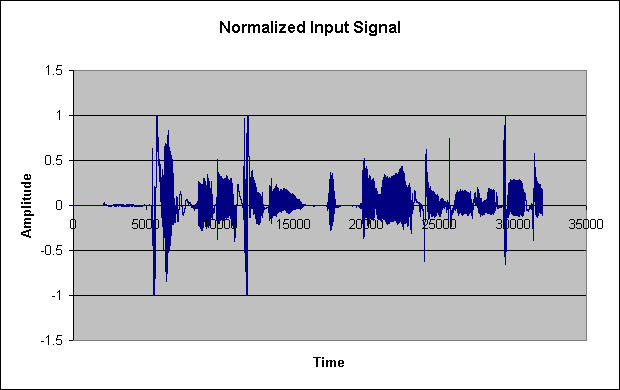
\includegraphics[width=400pt]{../graphics/graphs/wav-normalized.png}
	\caption{Normalization of aihua5.wav from the testing set.}
	\label{fig:prep-norm}
\end{figure}



\subsection{Endpointing}
\index{Preprocessing!Endpointing}
\index{Endpointing}
\index{Methodology!Endpointing}

The Endpointing algorithm got implemented in {\marf} as follows.
By the {\em end-points} we mean the local minimums and maximums
in the amplitude changes. A variation of that is whether to
consider the sample edges and continuous data points (of the same
value) as end-points. In {\marf}, all these four cases
are considered as end-points by default with an option to
enable or disable the latter two cases via setters or the \api{ModuleParams}
facility. The endpointing algorithm is implemented in \api{Endpoint}
of the \api{marf.Preprocessing.Endpoint} package and appeared in 0.3.0.5.

\subsection{FFT Filter}\label{sect:fft-filter}

The FFT filter is used to modify the frequency domain of the input sample in
order to better measure the distinct frequencies we are interested in.
Two filters are useful to speech analysis: high frequency boost, and low-pass
filter (yet we provided more of them, to toy around).

Speech tends to fall off at a rate of 6 dB per octave, and therefore the high
frequencies can be boosted to introduce more precision in their analysis.
Speech, after all, is still characteristic of the speaker at high frequencies,
even though they have a lower amplitude.  Ideally this boost should be performed
via compression, which automatically boosts the quieter sounds while maintaining
the amplitude of the louder sounds.  However, we have simply done this using a
positive value for the filter's frequency response.
The low-pass filter (\xs{sect:low-pass}) is used as a simplified noise reducer, simply cutting off
all frequencies above a certain point.  The human voice does not generate sounds
all the way up to 4000 Hz, which is the maximum frequency of our test samples,
and therefore since this range will only be filled with noise, it may be better
just to cut it out.

Essentially the FFT filter is an implementation of the Overlap-Add method of FIR
filter design \cite{dspdimension}.  The process is a simple way to perform fast convolution, by
converting the input to the frequency domain, manipulating the frequencies
according to the desired frequency response, and then using an Inverse-FFT to
convert back to the time domain. \xf{fig:fft-filter} demonstrates
the normalized incoming wave form translated into the frequency domain.

\begin{figure}
	\centering
	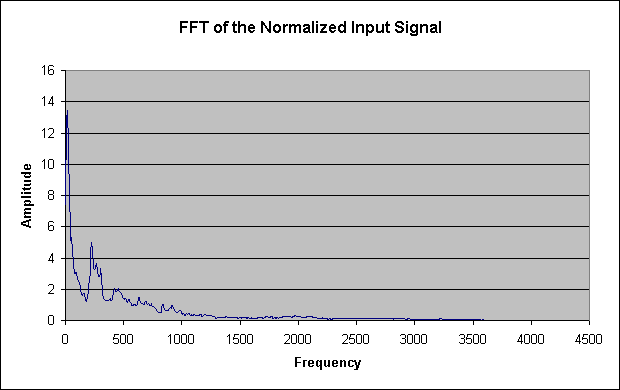
\includegraphics[width=400pt]{../graphics/graphs/fft.png}
	\caption{FFT of normalized aihua5.wav from the testing set.}
	\label{fig:fft-filter}
\end{figure}


The code applies the square root of the hamming window to the input windows
(which are overlapped by half-windows), applies the FFT, multiplies the results
by the desired frequency response, applies the Inverse-FFT, and applies the
square root of the hamming window again, to produce an undistorted output.

Another similar filter could be used for noise reduction, subtracting the
noise characteristics from the frequency response instead of multiplying,
thereby remove the room noise from the input sample.


\subsection{Low-Pass Filter}\label{sect:low-pass}

The low-pass filter has been realized on top of the FFT Filter,
by setting up frequency response to zero for frequencies
past certain threshold chosen heuristically
based on the window size where to cut off. We filtered out
all the frequencies past 2853 Hz.

\xf{fig:low-pass} presents an FFT graph of a
low-pass filtered signal.

\begin{figure}
	\centering
	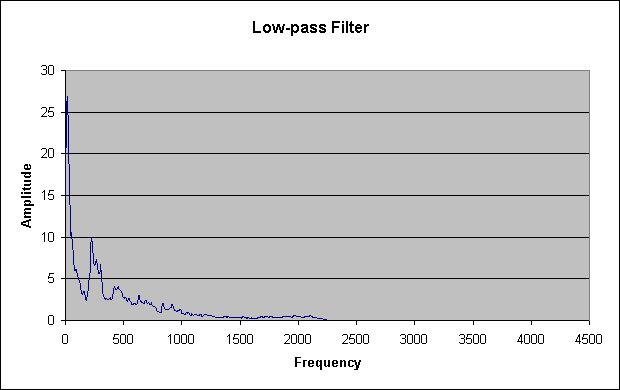
\includegraphics[width=400pt]{../graphics/graphs/low-pass-filter.png}
	\caption{Low-pass filter applied to aihua5.wav.}
	\label{fig:low-pass}
\end{figure}


\subsection{High-Pass Filter}
\index{High-Pass Filter}
\index{Filters!High-Pass Filter}

$Revision: 1.7 $

As the low-pass filter, the high-pass filter (e.g. is in \xf{fig:high-pass})
has been realized on top of the FFT Filter,
in fact, it is the opposite to low-pass filter, and filters out
frequencies before 2853~Hz.
The implementation of the high-pass filter can be found in
\api{marf.Preprocessing.FFTFilter.HighPassFilter}.

\begin{figure}
	\centering
	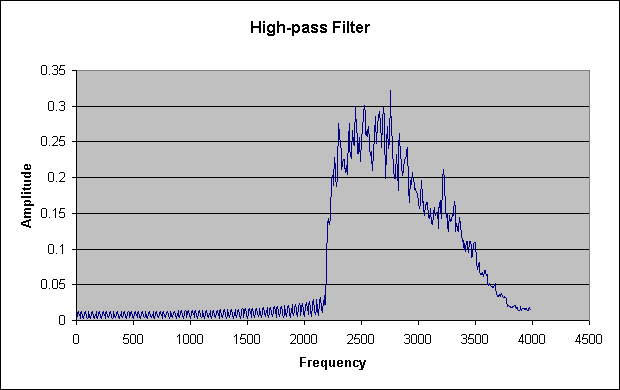
\includegraphics[width=400pt]{../graphics/graphs/high-pass-filter.png}
	\caption{High-pass filter applied to aihua5.wav.}
	\label{fig:high-pass}
\end{figure}

% EOF


\subsection{Band-Pass Filter}

Band-pass filter in {\marf} is yet another instance of an FFT Filter (\xs{sect:fft-filter}),
with the default settings of the band of frequencies of $[1000, 2853]$ Hz. See \xf{fig:band-pass}.

\begin{figure}
	\centering
	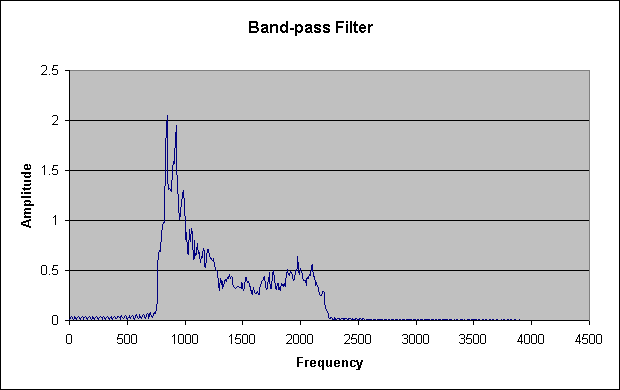
\includegraphics[width=400pt]{../graphics/graphs/band-pass-filter.png}
	\caption{Band-pass filter applied to aihua5.wav.}
	\label{fig:band-pass}
\end{figure}


\subsection{High Frequency Boost}
\index{High Frequency Boost}
\index{Filters!High Frequency Boost}

$Revision: 1.11 $

This filter was also implemented on top of the FFT filter to boost the high-end
frequencies. The frequencies boosted after approx. 1000~Hz by a factor
of $5\pi$, heuristically determined, and then re-normalized. See \xf{fig:high-boost}.
The implementation of the high-frequency boost preprocessor can be found in
\api{marf.Preprocessing.FFTFilter.HighFrequencyBoost}.

\begin{figure}
	\centering
	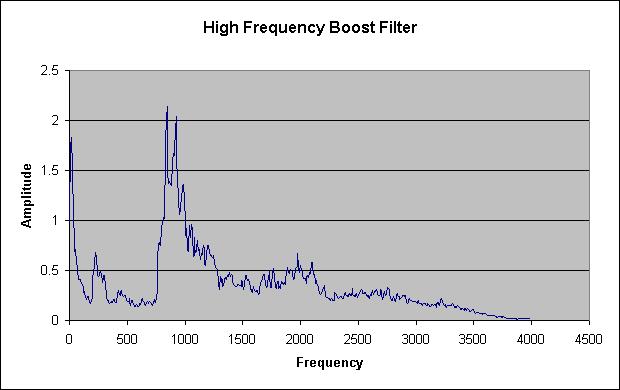
\includegraphics[width=400pt]{../graphics/graphs/high-frequency-boost.png}
	\caption{High frequency boost filter applied to aihua5.wav.}
	\label{fig:high-boost}
\end{figure}

% EOF


\subsection{High-Pass High Frequency Boost Filter}
\index{High-Pass High Frequency Boost Filter}
\index{Filters!High-Pass High Frequency Boost Filter}

$Revision: 1.2 $

For experimentation we said what would be very useful to do is
to test a high-pass filter along with high-frequency boost.
While there is no immediate class that does this, \api{MARF}
now chains the former and the latter via the new addition
to the preprocessing framework (in 0.3.0-devel-20050606)
where a constructor of one preprocessing module takes up another allowing
a preprocessing pipeline on its own. The results of this
experiment can be found in the Consolidated Results section.
While they did not yield a better recognition performance,
it was a good try to see. More tweaking and trying is
required to make a final decision on this approach as there
is an issue with the re-normalization of the entire input
instead of just the boosted part.

% EOF


\subsection{Noise Removal}

Any vocal sample taken in a less-than-perfect (which is always the case) environment will experience a certain
amount of room noise.  Since background noise exhibits a certain frequency characteristic,
if the noise is loud enough it may inhibit good recognition of a voice when the voice is
later tested in a different environment.  Therefore, it is necessary to remove as much
environmental interference as possible.

To remove room noise, it is first necessary to get a sample of the room noise by itself.
This sample, usually at least 30 seconds long, should provide the general frequency
characteristics of the noise when subjected to FFT analysis.  Using a technique similar
to overlap-add FFT filtering, room noise can then be removed from the vocal sample by
simply subtracting the noise's frequency characteristics from the vocal sample in question.

That is, if $S(x)$ is the sample, $N(x)$ is the noise, and $V(x)$ is the voice, all in the
frequency domain, then

\begin{center}$S(x) = N(x) + V(x)$\end{center}

Therefore, it should be possible to isolate the voice:

\begin{center}$V(x) = S(x) - N(x)$\end{center}

Unfortunately, time has not permitted us to implement this in practice yet.


% EOF
